\chaptertitle{1}{定投前的准备}
\setcounter{figure}{0}\setcounter{table}{0}
\subsection{如何省时省力打理好自己的财富}
{\heiti 投资要趁早}

提到投资理财，有很多刚开始工作或者手里没有多少钱的年轻朋友会这样想：现在手里本来就没多少钱，每个月随便花花就没了，想要投资理财，还是等以后有钱了再说吧。

但是这种想法，其实会有比较大的问题。因为投资需要时间，长期投资才能享受到复利的威力。投资要趁早。

我们举个例子，现在有早早、中中、晚晚三个人。

其中，早早最早开始投资理财，22岁大学毕业后就开始每个月定投1000元。

中中进行投资理财比较晚，27岁才开始自己的第一笔定投，但同样也是每个月定投1000元。

晚晚平时花钱大手大脚，一直到32岁才开始自己的第一笔定投，随后也是每个月定投1000元。

假设他们三个人定投的都是同一款年化收益率为8\%的投资品种。如果都是定投到60岁，他们可以分别积累下多少资产呢？

我们得到了图 \ref{fig:1-1} 。这是早早、中中、晚晚在几十年人生里，积累财富总量的走势图。

早早定投得最早，最后能够积累下大约310万元的资产。

\begin{figure}[htbp]
\centering
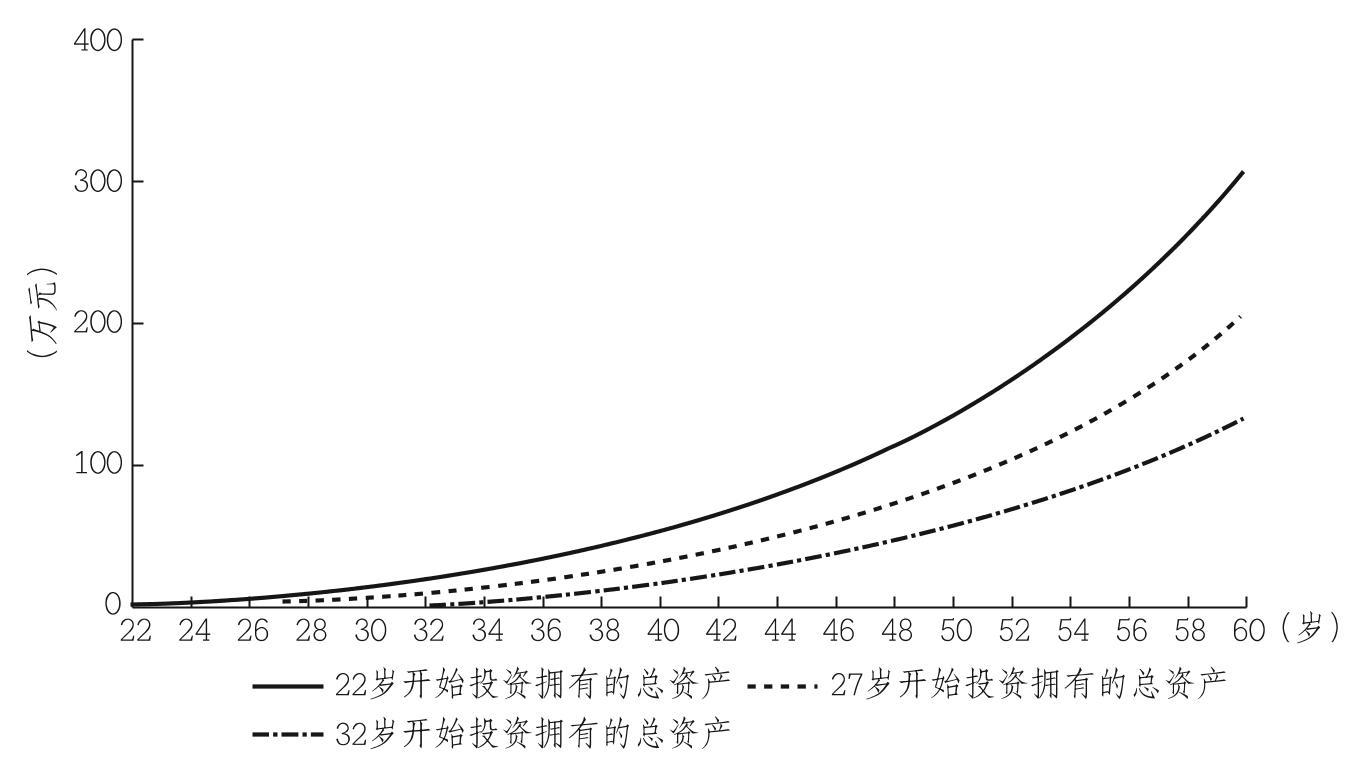
\includegraphics[width=\textwidth,height=0.82\textheight,keepaspectratio]{figure/图1.1.png}
\caption{在年化收益率为8\%的情况下，不同年龄开始投资到60岁的收益}\label{fig:1-1}
\end{figure}

中中积累的资产其次，最后能够积累下206万元的资产。

晚晚积累的资产最少，最后只有135万元的资产。

注意他们开始定投的时间，彼此之间相差只有5年。但最后积累的财富，相差七八十万元甚至上百万元。

在人生开始赚取收入的前5年，如果能越早开始投资理财，越到后期，积累财富的差距就会越大，想要赶上的难度也会越大。

我知道有些小伙伴会说：这个简单嘛，只要中中在27岁的时候，每个月能够多投资一些钱，不就能迎头赶上了吗？这样就算是晚投资了几年，应该也不会差多少吧？

那我们就来算算，如果你是中中，你比早早晚了5年开始投资，每个月你要多投入多少钱，才能赶得上早早。

计算的过程不详细讲了，直接给出结果：想要赶上早早，你必须在接下来的33年时间里，每个月投资1500元，也就是要每个月比早早多投资整整500元才行！

每个月要多投资50\%的本金，而且要整整33年的时间，你才能积累和早早一样多的财富。你可能觉得很委屈：我才晚了5年啊！

让我们再认真看看图 \ref{fig:1-1} ，在34岁之前，早早、中中、晚晚的财富没有特别大的差别，差距拉大是在34岁之后，复利的威力需要时间才能体现，时间越长，差异越大。

沃伦·巴菲特能够积累巨额财富，除了他具备别人难以企及的投资能力之外，他的投资生涯持续了60多年，到现在也没结束，也是重要的原因之一。而他的绝大部分财富，也是在60岁以后才拥有的。

所以，对于刚刚进入职场的小伙伴来说，投资理财，越早越好！一开始本金不多完全没关系，每个月就算拿出500元来投资，未来也有可能收获巨大的回报！

{\heiti 如何投资，才能让财富稳稳增长}

讲到这里，很多小伙伴要问：投资理财越早越好这个道理我懂，我就想获取长期稳定的投资收益，可是我该投资什么呢？

把钱存在银行，放在货币基金，连3\%的收益都没有，通货膨胀都跑不过！

买银行理财产品，有的门槛比较高，刚刚工作的人，每个月省下1000元不错了，要等好几年才买得起！

还有P2P（互联网借贷平台），出问题的太多了，没有安全感！

买股票？风险也不低，虽说找到好股票确实能让人获得超高收益，但是也要花大量时间来读公司年报、对公司进行分析估值，大部分刚进入职场的小伙伴都需要辛苦加班，怎么办？

还有更好的选择吗？有没有花费时间相对较少、长期收益较高、门槛较低、风险相对较低的办法？

当然有，答案就是定投指数基金，这也是本书想要重点介绍给大家的。

巴菲特曾经说过：“通过定投指数基金，一个什么都不懂的业余投资者，往往能够战胜大部分专业投资者。”

这句话告诉我们：投资指数基金的最佳策略，就是定投。每个月定期投入一定金额到指数基金，长期来看，让财富稳稳增长不是一件难事。

当然，定投哪只指数基金、什么时候定投、什么时候卖出，这些都是有技巧的，需要大家去学习和实践。

在接下来的章节中，螺丝钉也会讲到这些内容。

\subsection{养成3个理财好习惯，受益终身}
国内的财商教育是很落后的，很少有学校会给中小学生专门开设投资理财的课程。而且，现在独生子女多，通常是两代人三个家庭，去照顾一个孩子。家长很多时候对孩子的需求有求必应。

这就导致很多人在花钱上没有什么规划，也没有攒钱的意识：反正钱花不完，想要的时候也有人给，何必节约攒钱呢？

但是上了大学之后，孩子离开家庭，第一次手里有了不少数目的金钱可以支配，这钱怎么花，就成了一个问题。甚至这个问题比单纯地学习学校的知识还要重要。毕竟，大学学的东西可能毕业后没有用上，但是花钱和理财的习惯，是一辈子的事情。

{\heiti 好习惯一：把每月开支分成4份，避免把钱早早花完}

心理学上有个比较著名的实验。

{\kaishu 把糖放在桌子上，告诉一群小朋友，如果能不吃桌子上的糖，下午会再给一块。}

{\kaishu 然后实验员走开，观察小朋友的行为。}

{\kaishu 结果，大部分小朋友是无法忍耐到下午再吃的，他们会马上吃掉。只有一小部分小朋友坚持到下午再吃，因而获得了额外一块糖的奖励。}

这个实验告诉我们：人性是不耐的。

花钱也是如此。上班族每个月都会领工资，对于不耐的月光族来说，克制自己不乱花钱，是很困难的，很容易就在前半段时间把钱花光。

怎么改善这个现象呢？我们可以当工资发到手之后，立即把这个月用来支付日常开支的钱分成4份，每周分配一份，这样可以避免把钱早早地花完。

{\heiti 好习惯二：养成记账的习惯}

人的记忆力是有限的，很容易忘记之前发生的事情。

不过，好记性不如烂笔头。把以前的开销记录下来，这样我们就知道钱花到了哪里。现在有很多记账的App，通过手机记账很方便。

有了记账的习惯，知道自己的开销进度，知道钱花在了哪里，后面也更容易优化。

养成记账的习惯，会让你受益终身，很容易积累下财富。

{\heiti 好习惯三：做好预算}

第三个好习惯是，为将来的开支做好预算。

做预算已经是比较高级的技巧了，大部分人不一定有这个习惯。

我们知道预算部门是政府和企业很重要的部门，专门拟定未来的收支计划。而有这个习惯的个人并不多。

有了记账的习惯，我们就可以知道过去的时间段里，自己是怎么花钱的。

针对这些已经发生了的账单，我们就可以有针对性地进行增加收入、节省开支的预算规划。

对学生来说，主要是砍掉不必要的消费、优化必需的消费。

这里有朋友会觉得“砍掉消费项目”是非常困难的，怎么办呢？

其实有一个小窍门挺好用的，可以用“为物品贴上生命标签”这个方法。比如设定一杯星巴克咖啡=3小时生命，一件大衣=300小时生命（此处假定时薪为10元）等，这样，就可以很清楚地知道每一项消费的价值是多少，再问问自己这样值得吗。

答案立即就出来了。

熟练了之后，我们甚至可以比较精准地规划出自己下个月的开销是多少。

到了这一步，我们已经具备比较出色的消费观和财务技巧了。

\subsection{30岁之前，要不要买房、买车}
{\heiti 工作之后，要不要买车}

{\kaishu 钉大，大家都知道车子是消费品，尤其是贷款买的。那么在30岁这个人生阶段是不是应该去更多地购买资产而不是负债，包括贷款买房，因为一线城市房价那么高，房贷背负起来很累，而且也不是必需品，换成是你，你会怎么做？}

螺丝钉是这么看的，汽车是消费品。从买来开始使用算起，汽车就在不断贬值。

螺丝钉在北京住，也没有买车。出门需要的时候就打开叫车软件，随叫随到，经常还有优惠券可以用，折算下来比买车划算多了，也挺方便。所以，这种情况下，从财务角度打车就比买车划算一些。

不过，螺丝钉回老家的时候就觉得还是有车方便，因为不好叫车，公交也不发达。在老家生活，没有车的话会耽误大量的时间成本。这个时候有辆车会好一些。

所以，是否需要买车因人而异。

不过需要买车的时候，买个普通的便宜耐用的就好啦，没必要买太贵的。巴菲特的一辆“小破车”，也开了几十年呢。

房子就比较特殊了，它本身带有金融属性，能够抗通货膨胀。所以一个城市的房价，会随着居民人均收入的增长而增长，不像汽车贬值那么快。

不过确实没必要在年轻的时候就背负太高的房贷压力。在30岁之前，无论怎么去拼，大多数人都很难轻松负担一线城市的房价。这个在全世界都是如此，包括美国。

{\heiti 30岁之前，优先提升自己}

30岁之前，我们应该把更多的重心放在人力资产的培养。我们自己就是一个非常强大的资产。

根据美国布鲁金斯研究院2011年的调查数据，一个本科学历能带给我们的现金流，折算成金融领域的投资年复合收益率，竟高达15.2\%，远高于股票资产8\%～9\%的收益率。这也是我们要辛辛苦苦求学十几年、考好大学的原因。

同样是本科毕业，不同行业的工资也不同。像美国计算机工程毕业的本科生，平均年工资收入为6.1万美元，而有的专业则只有4万美元。

这些是从整体概率的角度得出的结果。好大学也有差学生，不过从整体上来看，一个好学历、好专业，给我们一辈子带来的收益是非常大的。

就算是上班后，我们也可以通过各种方式提升自己。例如银行的员工可以考相应的专业考试，比如CFA（特许金融分析师），这些证书可以在评职称的时候提供加分项，职称越高的员工月工资也会越高。拥有这类证书也是非常棒的、收益率很高、风险又非常低的资产。

再比如，看这本书学习投资理财。这本书能给我们带来知识，使我们未来现金流的提升不可估量。

21世纪什么最贵？人才，这才是全世界通用的硬资产。只不过提升自己比较辛苦，比较逆人性。

大家都明白这个道理。有些家长自己不怎么努力，但是对孩子严格要求，其实就是明白这个道理，但是不忍心对自己狠一点儿。

再说到买房。年轻人适不适合买房，买房的时候能不能从银行贷到款，其实银行是有比较通用的指标的：贷款人的月还款额/月收入，至少要低于50\%。

如果大幅高于这个数字，年轻人还是不要吃力供房了。一来生活质量会下降；二来背负这么高的贷款，人生也会丧失很多可能性。

{\heiti 年轻人租房，尽量住得离钱近一点}

如果不打算买房，那就需要考虑租房的事情。

有一段时间，北京、上海等城市的房租上涨成为一个热门话题。这些大城市的房价比较高，对很多刚工作的年轻人来说，无法负担直接买房的资金支出，租房是优先选择。

年轻人该如何租房呢？

记得螺丝钉刚毕业租房的时候，没什么经验，跟一个同事合租。第一次租的房子，在北京某公园附近，距离北京地铁五号线不远。

那一片有不少小区，房子本身一般，租房的人也鱼龙混杂，好在当时租房的价格还比较便宜。房子是一个一居室，不过客厅被简单地改造成一个卧室。

出租房子的是一个二房东，他把周围住户的房子收上来，进行简单的改造，或者打个隔断，这样就可以多出几个房间来出租了。

每天早上从租住的房子坐地铁去上班。五号线早上人非常多，刚开始没有经验，去地铁站的时候正好是上班高峰期，往往要等三四趟才能挤上去。

后来有经验了，早上早点儿走，5点多起床，6点多出门，这样地铁上人比较少，到单位后可以先去吃早餐。到了晚上，晚高峰也不想挤地铁，下班后就在单位附近吃个饭，看会儿书，待到晚一点再坐地铁回去。

虽然如此，但是每天来回路上所花的时间还是比较多的。所以后来实在不想在路上花费太长的时间，就打算退掉房子。

还记得当时二房东指着卧室门上的一个小窟窿说，这是你们弄出来的，要补400元，但是那个窟窿其实是一开始租房时就有的。协商未果，最后没办法，给了二房东200元，退掉了房子。

第二套房子租在了单位附近，也是合租。虽然租金跟第一套差不多，不过因为离市中心近了，面积小了许多，仅够放下一张床和一张书桌，居住条件也远不如第一套房子。

然而最大的好处就是：离单位近。这样，早上不用再那么着急，晚上也可以更早到家。有了更多的时间，就可以看更多的书。

当时螺丝钉开始对金融投资感兴趣，接触了很多金融产品的资料，买了很多金融类的书开始研究，也开始在网上写很多有关金融产品分析的文章。

第一套房子上下班通勤需要2个多小时，第二套房子上下班只需要20分钟。节约下来的1.5个小时，变成了螺丝钉脑中的知识，也变成了螺丝钉的一篇篇文章。

渐渐地，研究越来越深入，写的文章也越来越多，跟螺丝钉讨论的朋友也越来越多。

两年的时间里，就写了上百万字，看了上百本书。而完成这些，都是在工作之余，通过从各种地方节约下的时间来实现的。

虽然如今工作比从前更加忙碌了，但是，“挤出时间来看书”的习惯，还一直保留着。

房租是一笔消费，花出去就没有了。但是，“人”本身就是资产——人力资产，节约下时间在自己身上投资，是可以升值的。而且这个升值的空间，还非常大。

对年轻人来说，如果要租房，就选择在单位附近租住。如果不舍得花太多钱，那宁可面积小一点。通勤路上花太长时间，虽然可能会节约几百元，但浪费的时间是弥补不回来的。

时间很重要。节约下来的时间，不能浪费，如果用来学习，会加速我们的成长。

住得离工作近一点，住得离钱近一点。

在你觉得最重要的事情上，全力以赴！

这，就是螺丝钉眼中租房的秘诀。

\subsection{人到中年，如何规划好家庭消费}
{\kaishu 马上就40岁了，人到中年，我发现自己的中年财务危机很严峻。}

{\kaishu 跟年轻时相比，收入不见增长，可是花钱的地方越来越多：房贷、车贷、物业费、车位租金、养车钱、水电费、小孩学费、兴趣班和辅导班的费用、买菜钱等。}

{\kaishu 这些钱基本上就掏空了每月工资，都没钱孝敬父母，我该怎么办呢？}

这些问题相信大家都不陌生，许多中年人都会遇到这样的情况。螺丝钉也思考过该如何应对这样的困境，在此跟大家分享一下。

有的时候，我们不敢轻易换工作，因为身上背负着房贷和家庭其他开支。各种开销的压力大，孩子正是需要钱的时候，父母也是需要钱的时候。工作压力也大，中年人在公司基本上是中流砥柱或者业务主力。

人到中年，有点类似于一家企业到了转型期。比如说20世纪80年代的可口可乐（Coca-Cola），已经发展了很长时间，找不到新的业务增长点，可口可乐为了拓展业务，盲目进军了很多新的领域，甚至推出了可口可乐牌的酒，导致公司开销巨大，利润率下降。

后来，可口可乐重新聚焦于最核心的、能为公司带来现金流的业务，砍掉其他不赚钱的业务。同时，公司力争节俭，控制好每一笔开销。

概括来说，可口可乐转型的核心就在于聚焦主业，大力控制成本。

所以同样地，对于我们的小家庭而言，核心也主要在于这两个字：节流。

这里的节流是很有讲究的。螺丝钉把它总结为两句话：可选消费降级，必需消费走量。

{\heiti 可选消费降级}

如果把我们的日常开销区分一下，可以分成两类，一类是可选消费，一类是必需消费。

可选消费，是用来提高生活质量的。例如汽车、化妆品、最新款的手机、最新款的电脑，花费非常大的出境旅游等，都属于可选消费。有了它们，可以让我们更好地享受生活。但是如果经济能力达不到，没有它们，我们也可以继续生活。

很多时候，可选消费都是可以降级的。比如用不了最新款的比较贵的手机，用旧款的便宜点儿的手机也是可以的。旅游，没必要一定要出国，可以选择去一些花费少又好玩的地方，住不了五星级酒店，可以选择住民宿，或者去郊区逛逛公园、爬爬山也是不错的休闲娱乐方式。再比如汽车，买辆价格便宜的车也可以满足出行需求，或者是考虑跟同事朋友一起拼车上下班，分摊油费。

可选消费的特点是，很容易找到降级的替代方案。就好比手表，上到几十万的名表，下到几十元的普通表，都是有的，都能满足看时间的基本需求。我们可以根据自己的实际经济能力选择合适的消费品。

{\heiti 必需消费走量}

必需消费，是维持日常生活的消费。衣食住行，都算是必需消费。必需消费的单价都不高，属于日常消耗品。

通常来说，必需消费品可以一次性大量买入，这样会划算一些。比如超市或者电商做优惠活动的时候多买一些，或使用优惠券或者满减券等，这样会比平时买更便宜。而这些必需消费品又是每天都在不断消耗的，所以不怕买了不用反而浪费钱。当然，也不要囤太多。一次性买特别多的东西囤着，有时会起到反作用，吞噬我们的流动资金。基本上，一次囤一个季度的必需消费品就可以了。像很多电商每隔一段时间就做优惠活动，我们不用担心后面买不到便宜的商品。

{\heiti 聚焦主业}

做好以上两方面之后，我们还需要聚焦主业。聚焦主业也可以帮助我们减少不必要的开销。

比如说孩子的教育。螺丝钉以前见到过一些家长，给孩子同时报了钢琴、舞蹈、书法、英语等多个辅导班。虽然说在教育上进行投资是非常划算的，长期来看，在教育上投入的资金回报率非常高，但是，人的精力是有限的，孩子也一样。在任何一个领域，想要取得成就，都得投入大量的时间和精力。报太多的兴趣班，每一个都学，可能每一个都学不好，所以给孩子报辅导班、兴趣班，不能盲目地去报，要聚焦主业。

想想孩子对什么方面更感兴趣，孩子以后要走哪条路，哪些技能可以帮助孩子在这条路上走得更远，再围绕这个方向来投入时间和金钱，而其他的非主营业务，都可以砍掉。

我们在做事业的时候也是如此。比如说工作中会面对很多不同的项目，可能每一个项目都是不错的，但人的精力有限，选择一个自己擅长的核心项目来投入精力，比所有项目都做效果要更好。

每一个项目都做，可能每一个项目都做不好。认清自己要做的是什么，聚焦主业。

{\heiti 定期检查}

最后一点，我们还需要定期检查。

人都是有惰性的。由俭入奢易，由奢入俭难。按照人的惰性，都是倾向于花钱越来越多的，所以我们需要定期为家庭开销做好规划。如果不定期检查，家庭开销可能不知不觉地就提上去了。定期检查可以帮助我们及时改进。别等到一年过去了，到年底才发现家里没攒下一分钱。夫妻俩定期合计合计，甚至可以节约下超过30\%的钱。

\subsection{穷人思维和富人思维，决定你一生的财富}
我们经常说到穷人思维和富人思维，那穷人思维和富人思维到底是什么呢？

这里螺丝钉讲一个小故事。

{\heiti 比尔·盖茨慈善基金会扶贫的故事}

大家都知道，每年国家都会有一些定向扶贫的项目。比如说养殖类项目，向贫困家庭赠送鸡和鸭，通过养鸡、鸭获得鸡蛋、鸭蛋等方式来提高其收入。比如说种植类项目，帮助贫困家庭种植橘子、核桃等树木，通过出售所结果实来提高其收入。

从某种意义上来说，这就是给贫困家庭提供了一个可以产生现金流的资产。性质上，跟我们投资理财是一样的，都可以产生现金流。

这种方法其实是全世界通用的。

以前读比尔·盖茨慈善基金会的一些文章，比尔·盖茨（Bill Gates）每年会给贫困家庭送小鸡。

养鸡是一个见效非常快的脱贫方法。鸡是一种能产生现金流的资产，所以在全世界范围，养鸡是贫困家庭脱贫致富的常见选择。

比尔·盖茨的慈善基金会深谙其中的道理。

{\kaishu 我和我的同事们在长期的基层工作过程中，遇到了很多生活费每天不足2美元的人。我多年的经验是，养鸡可以改变这些人的生活。}

{\kaishu 一个非洲农民可以从养5只鸡开始，3个月后，其就有了一个40只鸡的小鸡群。最终，在非洲养殖的每只鸡以西方批发价5美元的销售价出售后，该农民可以每年赚取超过1000美元的收入，超过该地每年收入约700美元的极端贫困水平。}

{\kaishu 你可能会认为养鸡的目的是吃鸡蛋，但是，正如我们在这里讨论的，很多农民发现不吃鸡蛋更有经济意义：让鸡蛋孵化，提高鸡的出栏率，然后把鸡卖掉，用卖鸡得到的这笔钱来购买食物。}

{\kaishu 鸡的养殖相对便宜和简单可行，鸡只需要住所、药品和食物。鸡可以吃它们在地面上发现的任何食物品种。}

这就是最简单的“持有资产致富”的道理。比尔·盖茨基金会每年会投放超过10万只小鸡到贫困地区。

那是不是告诉贫困家庭要养鸡，给他们送小鸡，事情就解决了呢？其实也不是。人性是不耐的。即使是养鸡这种扶贫方法，也会遇到难题。

之前有关注螺丝钉的朋友说过他扶贫时的案例。

{\kaishu 关于扶贫，我们当地有个笑话流传，就是县长去扶贫，给一家贫困户买了很多小鸡叫他们养大。过了几天这家贫困户去县政府找县长，县长不在，秘书问有什么事，贫困户答：“光给我买了小鸡没用，小鸡吃啥？没有饲料。”秘书只得送了很多鸡饲料去。}

{\kaishu 又过了3个月，县长去看这家贫困户，发现小鸡和饲料都不见了，贫困户说小鸡比较难喂，吃了。}

{\kaishu 由此我联想到投资也是如此，为什么很多人没有最终富有，那是因为他们没有忍受饥寒交迫、坚持艰苦奋斗的耐心。}

{\kaishu 所以要想脱贫，就必然得忍受很久一段时间的贫穷，而这种品质叫作坚守！}

还有朋友分享了以下案例。

{\kaishu 扶贫是一个沉重的话题，大约20年前他本人也直接参与过扶贫工作，也是着眼于提高贫困群体的“造血”功能，结合农业区的实际，提供了鸡仔、猪仔等给贫困群体养殖。}

{\kaishu 愿望是美好的，但现实是残酷的。提供鸡仔、猪仔后，饲料、养殖方式、卫生防疫等问题接踵而至，不少人半路放弃了。坚持到最后的群众，扶贫人员还要帮助他们把产品，如鸡蛋、猪肉都卖出去。}

{\kaishu 两年之后，他们总结的结果是，对于贫困人员，最好是以富带贫，通过发展产业项目，把贫困人员吸纳进来，让他们从事力所能及的工作，通过报酬来解决贫困问题。}

{\kaishu 否则，只能养懒汉。}

这就是典型的穷人思维：不耐和懒惰。

{\heiti 穷人思维：不耐和懒惰}

有的人贫穷是因为极端没有耐心，他们甚至无法等到生长周期短的鸡成长起来。对这些人来说，持有一周就是“长期投资”了。如果让这些人去做股票投资，也是只有持有几天的耐心。极端没有耐心，让这些人无法等待资产产生现金流。任何情况下，消费都比投资更容易。因为消费不需要等待，是一种即时享受。但是同样的钱，去做任何一种投资，都需要时间的沉淀。这就需要我们有足够的耐心。

还有一类人贫穷则是因为懒惰。懒惰的意思是不想贡献人力资产，只想不劳而获。

人人都想财务自由，但是如果自己本身的资产比较少，那么通过劳动，用自己的人力资产去赚钱，是必需的过程。

这也是为何大多数人都需要上班的原因。我们自己也是一个可以产生现金流的资产，自己不努力，这个资产的价值就会大大缩水。

正如一段相声里讲的：“但凡要饭的，没有要早饭的，因为他要是能早起，就不至于要饭。”

人性的不耐和懒惰，就是穷人思维的核心。

我们想要变得富有，就不能犯同样的错误。

{\heiti 投资者笔记}

\begin{itemize}
\item {\kaishu 投资要趁早。}
\item {\kaishu 30岁之前，优先提升自己。如果要租房，尽量住得离工作近一点，住得离钱近一点。}
\item {\kaishu 人到中年，规划好家庭消费的核心在于：可选消费降级，必需消费走量。}
\item {\kaishu 人性的不耐和懒惰，是人们陷入贫穷的根本原因。我们想要变得富有，就不能犯同样的错误。}
\end{itemize}

